\documentclass[conference]{IEEEtran}
\IEEEoverridecommandlockouts

% Packages used:
\usepackage{hyperref}
\usepackage{cite}
\usepackage{amsmath,amssymb,amsfonts}
\usepackage{algorithmic}
\usepackage{graphicx}
\usepackage{textcomp}
\usepackage{xcolor}

\usepackage{listings}
\usepackage{xcolor}

\usepackage{tikz,amsmath}
\usetikzlibrary{shapes.geometric, arrows, fit, backgrounds}

\tikzstyle{process} = [rectangle, minimum width=2.5em, minimum height=2.5em, text centered, draw=black, fill=gray!10]
\tikzstyle{startend} = [ellipse, minimum width=2.5em, minimum height=1.5em, text centered, draw=red, fill=gray!10]
\tikzstyle{arrow} = [thick,->,>=stealth]

\lstdefinestyle{json}{
  basicstyle=\ttfamily\footnotesize,
  breaklines=true,
  frame=single,
  backgroundcolor=\color{gray!10},
  showstringspaces=false
}

\lstdefinestyle{cstyle}{
  language=C,
  basicstyle=\ttfamily\footnotesize,
  breaklines=true,
  frame=single,
  backgroundcolor=\color{gray!10},
  showstringspaces=false,
  keywordstyle=\color{blue},
  commentstyle=\color{green!50!black},
  stringstyle=\color{orange}
}

\def\BibTeX{{\rm B\kern-.05em{\sc i\kern-.025em b}\kern-.08em
    T\kern-.1667em\lower.7ex\hbox{E}\kern-.125emX}}

\begin{document}

%------------------------------------------------------------------
% Title Page
%------------------------------------------------------------------
\title{Leveraging Artificial Intelligence for Automated validation of C code}


\author{\IEEEauthorblockN{1\textsuperscript{st} Given Name Surname}
\IEEEauthorblockA{\textit{dept. name of organization (of Aff.)} \\
\textit{name of organization (of Aff.)}\\
City, Country \\
email address or ORCID}
\and
\IEEEauthorblockN{2\textsuperscript{nd} Given Name Surname}
\IEEEauthorblockA{\textit{dept. name of organization (of Aff.)} \\
\textit{name of organization (of Aff.)}\\
City, Country \\
email address or ORCID}
\and
\IEEEauthorblockN{3\textsuperscript{rd} Given Name Surname}
\IEEEauthorblockA{\textit{dept. name of organization (of Aff.)} \\
\textit{name of organization (of Aff.)}\\
City, Country \\
email address or ORCID}
\and
\IEEEauthorblockN{4\textsuperscript{th} Given Name Surname}
\IEEEauthorblockA{\textit{dept. name of organization (of Aff.)} \\
\textit{name of organization (of Aff.)}\\
City, Country \\
email address or ORCID}
\and
\IEEEauthorblockN{5\textsuperscript{th} Given Name Surname}
\IEEEauthorblockA{\textit{dept. name of organization (of Aff.)} \\
\textit{name of organization (of Aff.)}\\
City, Country \\
email address or ORCID}
\and
\IEEEauthorblockN{6\textsuperscript{th} Given Name Surname}
\IEEEauthorblockA{\textit{dept. name of organization (of Aff.)} \\
\textit{name of organization (of Aff.)}\\
City, Country \\
email address or ORCID}
}

\maketitle

\begin{abstract}
The objective of this work is to create an automated unit testing solution for a codebase using LLMs (Large Language Models), LangChain, LangGraph, Python. A multi-agent system was created to automatically create unit tests for AMD’s openSIL (Advanced Micro Devices’ Open-Source Silicon Initialization Library) codebase. The codebase consisted of silicon initialization code and was built using the EDK II (Extensible Firmware Interface Development Kit) Build System. Performance is measured by line coverage of the unit test as the goal is to maximize line coverage. LLMs can be divided into two categories, reasoning and non-reasoning models. Previous works have explored unit testing capabilities of non-reasoning models. For this project, we focus specifically on utilizing reasoning models such as OpenAI o3 to create unit tests. In evaluation, the system compiled 73 out of 76 functions and reached an average line coverage of 84\%.  After adding LCA (Line-Coverage Analysis) and a line-coverage step that target missed lines, line coverage rose to 99\% on a second batch of 50 functions. By category, small and medium functions were the most consistent, while big and XFER/Ip2Ip ones required more time, effort, and edits. 
\end{abstract}

\section{Introduction}
Software quality assurance relies significantly on rigorous testing, and unit testing plays a pivotal role by assessing individual units of source code in isolation. Unit tests help identify errors early, improving software maintainability and reliability. A variety of metrics have traditionally been employed to evaluate the effectiveness of unit testing, notably line coverage, branch coverage, and function coverage [1][3]. Despite their critical role, writing comprehensive and effective unit tests manually can be resource-intensive, error-prone, and challenging, especially in complex, dependency-heavy systems like firmware. 

Automating unit test generation presents an attractive solution to address these challenges. Previous research on automated unit test generation has largely focused on symbolic execution, static analysis, and search-based methods. However, these techniques often struggle to scale with complex or low-level systems, such as firmware codebases, which involve intricate interactions with hardware and extensive pointer manipulation. Recently, large language models (LLMs) have emerged as a promising alternative for automated unit testing, offering human-like readability and a flexible approach to code generation [2][4][5]. 

Existing work using LLMs for unit test generation has predominantly employed non-reasoning models—those lacking explicit training to enhance reasoning capabilities through methods such as reinforcement learning. These non-reasoning models have achieved notable success but exhibit significant limitations in scenarios requiring complex reasoning or handling nuanced, low-level coding tasks [6][7]. Consequently, there is a pressing need to explore reasoning-based LLMs, which leverage explicit training techniques such as Chain-of-Thought (COT) reasoning to achieve higher accuracy and deeper code understanding. 

In this work, we address the limitations of existing approaches by specifically utilizing reasoning-based LLMs to automate unit testing for AMD’s OpenSIL (Open-Source Silicon Initialization Library) firmware codebase. OpenSIL is characterized by structured yet highly interdependent functions, making it an ideal candidate for automated testing strategies. Our goal is to maximize line coverage while reducing manual effort in test generation.  

To the best of our knowledge, this is the first paper exploring the application of reasoning-enhanced LLMs to firmware unit testing, marking an important step towards broader adoption and refinement of automated testing methodologies

\section{Background}
Unit testing remains a cornerstone of software quality assurance, enabling early detection of defects and improving long-term maintainability. Its effectiveness is often quantified using metrics such as line coverage, branch coverage, and function coverage [1][3]. While these metrics have been widely studied in high-level software systems, achieving high coverage in firmware or low-level C/C++ environments presents unique challenges. Firmware typically operates under strict build constraints, involves pointer-intensive logic, and interacts directly with hardware registers, making isolation of testable units more difficult. Prior firmware testing work has explored static analysis and hardware abstraction to mitigate these challenges, but such methods remain largely manual, requiring significant engineering effort and domain expertise. 

Automated unit test generation has traditionally relied on symbolic execution, mutation testing, and search-based approaches, each with trade-offs in scalability, completeness, and runtime cost. Symbolic execution offers path exploration guarantees but struggles with the state-space explosion common in hardware-interfacing code. Search-based methods, while adaptable, can produce brittle tests that break with minor code changes. As a result, most prior automation efforts have concentrated on high-level managed languages such as Java or Python [2][4][5], with only limited work targeting compiled-language firmware code [3][8][9]. The gap is particularly evident in environments where dependencies span multiple modules and where hardware APIs require specialized mocking or stubbing. 

In recent years, Large Language Models (LLMs) have emerged as an alternative for automated test generation, producing human-readable code and adapting flexibly to various programming paradigms [6][7][13]. However, most prior research has employed non-reasoning models, which—while capable of chain-of-thought reasoning—lack the explicit optimization for complex, multi-step problem solving seen in reasoning-tuned models [9]. Non-reasoning models show promise but often exhibit low compilation success rates, incomplete dependency handling, and reduced coverage in pointer-heavy, low-level scenarios. In contrast, reasoning-enhanced models such as OpenAI’s O3 [10] and DeepSeek’s R1 incorporate reinforcement learning and CoT reasoning to improve logical consistency and multi-step planning, making them strong candidates for complex code generation tasks. 

This work applies reasoning-enhanced LLMs to the AMD OpenSIL firmware codebase—a structured but dependency-rich silicon initialization library—and evaluates their ability to automatically generate effective unit tests. The main contributions are: 

i. Parsing complexity management – Development of a parsing engine to extract and represent deep and shallow dependencies, enabling LLM agents to navigate intricate firmware code structures.

ii. Utilization of reasoning models – Application of reasoning-tuned LLMs for automated unit test generation in a pointer-intensive, hardware-interfacing environment.

iii. Firmware-specific behavioral evaluation – Empirical measurement of compilation success rates, coverage metrics, and functional correctness when reasoning-based LLMs are applied to firmware codebases.

\subsection{Codebase Overview}
OpenSIL (Open-Source Silicon Initialization Library) is an open-source, modular firmware library primarily designed to initialize and configure AMD silicon platforms. It abstracts hardware-specific initialization logic, facilitating reuse across different firmware implementations, including coreboot and UEFI-based systems. 

The codebase consists of distinct layers:

{\small
\begin{itemize}
\item Platform Abstraction Layer (PAL): Provides standardized interfaces to abstract platform-specific functionalities, enhancing portability and code reuse. 

\item Silicon Initialization Modules: Includes functions that handle detailed initialization tasks for components like memory controllers, security processors, and chipset interfaces. These modules contain functions with highly specific input-output behavior, ideal candidates for automated testing. 

\item Configuration and Policy Management: Encapsulates configurable parameters and policies influencing initialization logic, enabling flexible adaptation to varied hardware configurations. 

\end{itemize}
}

Given the complex yet structured nature of OpenSIL functions, our research employs Large Language Models (LLMs) to automatically generate comprehensive unit tests. Leveraging clear function definitions and documented behaviors in OpenSIL, LLM-driven test generation aims to increase testing coverage, detect edge-case failures, and improve overall firmware robustness without extensive manual effort. 

The codebase includes several unit tests. A unit test consists of the following files:

i. (Optional) Header file: The header file could include declarations and/or other header files which may be needed for the unit test. The same could have also been written directly in the source file so this file is not always included. 

ii. Source file: The source file consists of the actual unit testing logic. It includes any necessary stubs, mocks, etc. It contains the code for one or more test iterations. 

iii. JSON file: The JSON file consists of the names of the test iterations and optionally their descriptions. The test iterations match with a single unit test with its own input data. 

iv. INF file: The inf files contains the configuration for the unit tests. It describes the needed packages, library classes, and source files. The unit test cannot be successfully compiled and dispatched without proper configuration of this file. 

\subsection{Characteristics of Functions}
Functions in the OpenSIL codebase exhibit specific characteristics that influence the approach required to test them. For example, certain functions may require mock implementations. In such cases, the agent should first check the pre-existing mock library and reuse the mocked function if it exists. If it does not, the agent should be capable of generating the necessary mock itself. The following subsections describe the main function characteristics and the testing strategies used for each.

\subsubsection*{\textbf{Require Stubs/Mocks/Fakes}}
Some functions call other functions included from different source files. Because unit tests are executed in isolation, these external dependencies are not available and must therefore be stubbed, mocked, or faked. Furthermore, all functions called within the source file must also be stubbed, mocked, or faked, even those not directly under test, otherwise the file cannot be built.  

To handle this, the agent should verify whether the required function is present in the Stub/Mock/Fake libraries. If it is, the corresponding header file must be included in the unit test, and the library itself added as a dependency in the INF file. If the required function is not present, the agent should determine whether to create a stub, mock, or fake and generate it accordingly.

\subsubsection*{\textbf{Returns a Value}}
Some functions return a value via a return statement. In such cases, the agent should identify the return type by analyzing the function signature and then verify correctness by asserting that the return value matches the expected result.

\subsubsection*{\textbf{Returns a Value Through a Pointer Argument}}
Other functions return values through pointer arguments passed to them. These cases can be handled by analyzing the source code and consulting the function documentation to determine how the output should be validated.

\subsubsection*{\textbf{Utilizes an XFER Table}}
Certain functions rely on an XFER table, which is a data structure containing function pointers. The table is obtained by calling \texttt{SilGetCommon2RevXferTable}, which provides it via a pointer. Functions in the XFER table are external dependencies and must be mocked appropriately. An example is shown in Figure ~\ref{fig:xfer_struct} and  Figure ~\ref{fig:xfer_example} below.

{ \small
\begin{figure}[hbt!]
  \centering
  \begin{lstlisting}[style=cstyle]
typedef struct {
    DF_FABRIC_REGISTER_ACC_READ   DfFabricRegisterAccRead;
    DF_FABRIC_REGISTER_ACC_WRITE  DfFabricRegisterAccWrite;
    .
    .
    .
    DF_HAS_FCH                    DfHasFch;
    DF_HAS_SMU                    DfHasSmu;
} DF_COMMON_2_REV_XFER_BLOCK;

DF_COMMON_2_REV_XFER_BLOCK DfCmn2RevPhxXfer = {
    .DfFabricRegisterAccRead = DfXFabricRegisterAccRead,
    .DfFabricRegisterAccWrite = DfXFabricRegisterAccWrite,
    .
    .
    .
    .DfHasFch = PhxHasFch,
    .DfHasSmu = PhxHasSmu
};
  \end{lstlisting}
  \caption{Retrieving the \texttt{XFER} table into the \texttt{CcxXfer} variable and calling a function from it.}
  \label{fig:xfer_struct}
\end{figure}
}

To test these functions, we can call \texttt{MockSilGetCommon2RevXferTableOnce} to override the return value with a custom XFER table.

\begin{figure}[hbt!]
  \centering
  \begin{lstlisting}[style=cstyle]
extern DF_COMMON_2_REV_XFER_BLOCK DfCmn2RevPhxXfer;
extern DF_IP2IP_API DfIp2IpApiPhx;

SIL_STATUS
InitializeApiDfXPhx (
  SIL_CONTEXT  *SilContext
  )
{
  SIL_STATUS Status;

  // Set Cmn2Rev table for DF
  Status = SilInitCommon2RevXferTable(SilContext, SilId_DfClass, &DfCmn2RevPhxXfer);
  if (Status != SilPass) {
    return Status;
  }

  // Set Ip2Ip API for DF
  return SilInitIp2IpApi(SilContext, SilId_DfClass, (void *) &DfIp2IpApiPhx);
}
  \end{lstlisting}
  \caption{Retrieving the \texttt{XFER} table into the \texttt{CcxXfer} variable and calling a function from it.}
  \label{fig:xfer_example}
\end{figure}

\subsubsection*{\textbf{Utilizes Ip2Ip Functionality}}
Similar to XFER tables, some functions use an \texttt{Ip2Ip} structure that contains function pointers. These are retrieved by calling \texttt{SilGetIp2IpApi}. The functions in the returned table are external dependencies and must also be mocked.  

To test these functions, the agent can call \texttt{MockSilGetIp2IpApiOnce} to substitute the return value with a custom Ip2Ip table. An example is shown in Figure ~\ref{fig:ip2ip_example}.

\subsubsection*{\textbf{Small Functions}}
Small functions are typically fewer than 20 lines of code. They usually contain only a limited number of branches and low complexity, making them faster and easier to test.

\subsubsection*{\textbf{Medium Functions}}
Medium functions range from 20 to 70 lines of code. They may involve more branching logic and often incorporate structures such as Ip2Ip or XFER tables, increasing the complexity of testing.

\subsubsection*{\textbf{Large Functions}}
Large functions contain more than 70 lines of code and exhibit high complexity with many branching paths. Testing them thoroughly requires careful analysis to ensure all branches are covered.

\subsubsection*{\textbf{Static Functions}}
Static functions cannot be called from outside their source file, which prevents them from being directly tested by unit test code. As such, they represent an edge case in unit testing.

\begin{figure}[hbt!]
  \centering
  \begin{lstlisting}[style=cstyle]
  RAS_IP2IP_API *RasApi; 
  Status = SilGetIp2IpApi (SilId_RasClass, (void **)&RasApi); 
  if (Status != SilPass) { 
    XPRF_TRACEPOINT (SIL_TRACE_ERROR, "RAS API not found!\n"); 
    return Status; 
  } 
  RasApi->ProgramCoreMcaIpIdInstanceId (RasCpuInfo); 
  \end{lstlisting}
  \caption{Retrieving the \texttt{Ip2IpApi} into the \texttt{RasApi} variable and calling a function from it.}
  \label{fig:ip2ip_example}
\end{figure}

\begin{figure}
\centering
\hfill\\
{\scriptsize
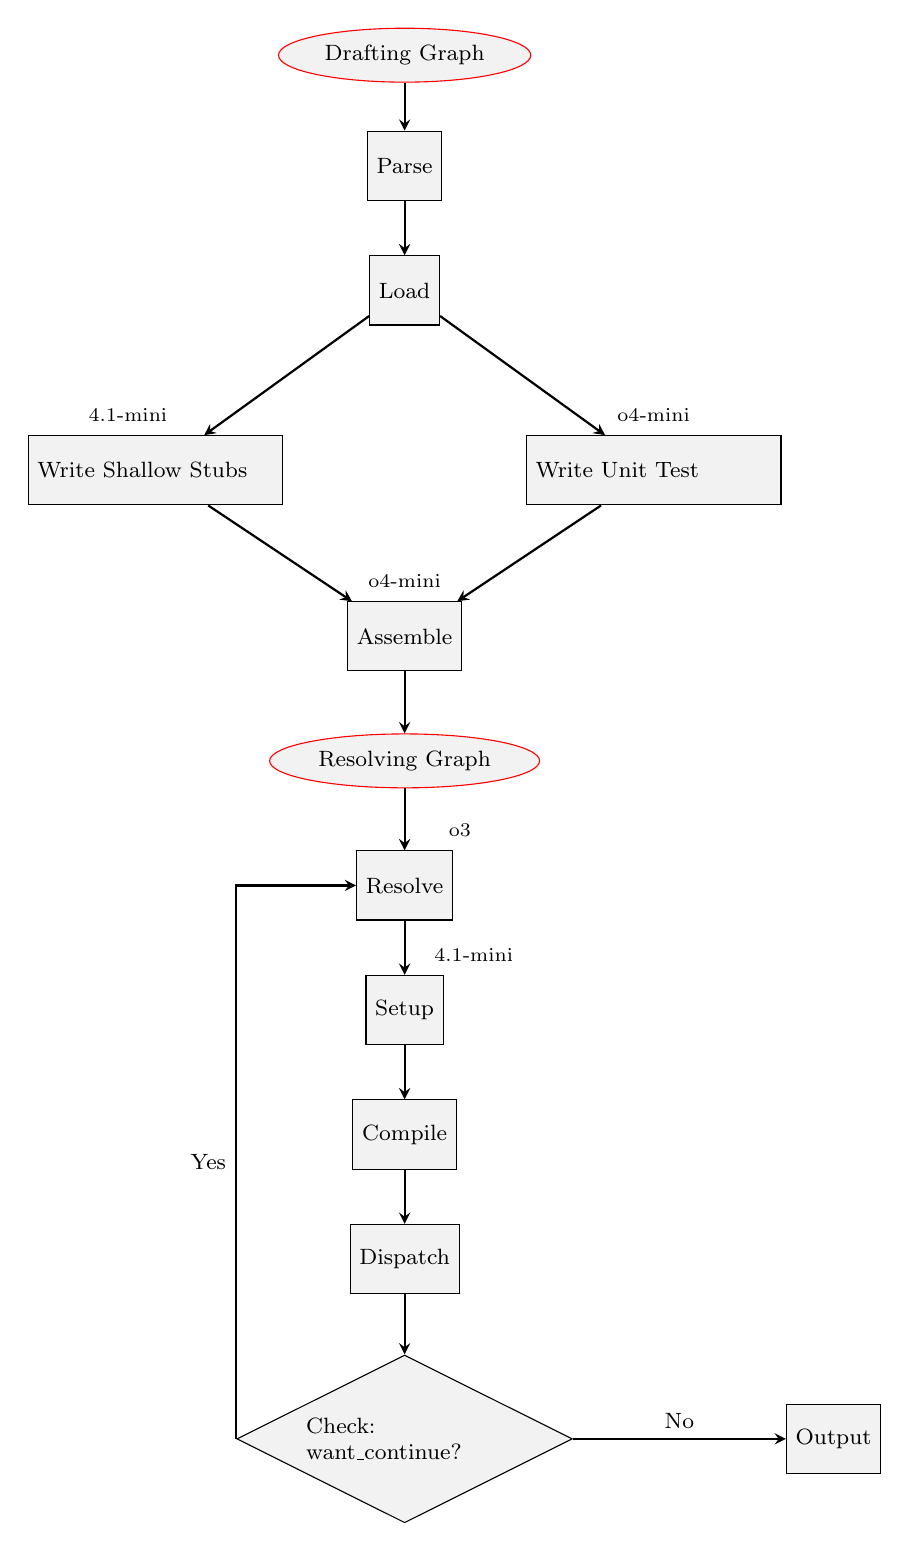
\begin{tikzpicture}[node distance=2.5em, every node/.style={font=\footnotesize}, 
  on background layer/.style={}]

% --------- Drafting Graph ----------
\node (DGtitle) [startend] {\footnotesize Drafting Graph};
\node (PARSE)   [process, below of=DGtitle, yshift=-1.5em] {\footnotesize Parse};
\node (LOAD)    [process, below of=PARSE, yshift=-2.0em]   {\footnotesize Load};

% Keep these compact so they fit the column
\node (WSS)     [process, below of=LOAD, yshift=-4.0em, xshift=-9em]{\parbox[t][][t]{3.0cm}{\footnotesize Write Shallow Stubs}};
\node (WUT)     [process, below of=LOAD, yshift=-4.0em, xshift=9em]{\parbox[t][][t]{3.0cm}{\footnotesize Write Unit Test}};
\node (WUT_NOTE) [above of=WUT, yshift=-0.5em, xshift=0em, draw=none, fill=none] {\scriptsize o4-mini};
\node (WSS_NOTE) [above of=WSS, yshift=-0.5em, xshift=-1em, draw=none, fill=none] {\scriptsize 4.1-mini};
\node (ASM)     [process, below of=LOAD, yshift=-10.0em]{\footnotesize Assemble};
\node (ASM_NOTE) [above of=ASM, yshift=-0.5em, xshift=0em, draw=none, fill=none] {\scriptsize o4-mini};

% --------- Resolving Graph ----------
\node (RGtitle) [startend, below of=ASM, yshift=-2.0em] {\footnotesize Resolving Graph};


\node (RESOLVE) [process, below of=RGtitle, yshift=-2.0em] {\footnotesize Resolve};
\node (RESOLVE_NOTE_TXT) [above of=RESOLVE, yshift=-0.5em, xshift=2em, draw=none, fill=none] {\scriptsize o3};
\node (SETUP)   [process, below of=RESOLVE, yshift=-2.0em] {\footnotesize Setup};
\node (SETUP_NOTE) [above of=SETUP, yshift=-0.5em, xshift=2.5em, draw=none, fill=none] {\scriptsize 4.1-mini};
\node (COMPILE) [process, below of=SETUP,  yshift=-2.0em] {\footnotesize Compile};
\node (DISPATCH)[process, below of=COMPILE,yshift=-2.0em] {\footnotesize Dispatch};

% Make the decision compact and centered
\node (CHECK)   [diamond, draw=black, fill=gray!10, text width=2.5cm, aspect=2,
                 below of=DISPATCH, yshift=-4.0em]{\parbox[t][][t]{3.0cm}{\footnotesize Check: want\_continue?}};
\node (OUTPUT)  [process, right of=CHECK, xshift=13.0em] {\footnotesize Output};

% Edges (Drafting)
\draw [arrow] (DGtitle) -- (PARSE);
\draw [arrow] (PARSE) -- (LOAD);
\draw [arrow] (LOAD) -- (WSS);
\draw [arrow] (LOAD) -- (WUT);
\draw [arrow] (WSS)  -- (ASM);
\draw [arrow] (WUT)  -- (ASM);

% Edges (Bridge + Resolving)
\draw [arrow] (ASM) -- (RGtitle);
\draw [arrow] (RGtitle) -- (RESOLVE);
\draw [arrow] (RESOLVE) -- (SETUP);
\draw [arrow] (SETUP) -- (COMPILE);
\draw [arrow] (COMPILE) -- (DISPATCH);
\draw [arrow] (DISPATCH) -- (CHECK);
\draw [arrow] (CHECK) -- node[anchor=south]{No} (OUTPUT);

% Loop back on Yes (tight bend to stay within the column)
\draw [arrow] (CHECK.west) |- node[anchor=east,pos=0.25]{Yes} (RESOLVE);

\end{tikzpicture}}
\caption{DraftingGraph and ResolvingGraph workflow (nodes, iteration, and decision).}
\label{fig:multiagent_graph}
\end{figure}

\section{Related work}
Large language models (LLMs) have quickly become a compelling alternative to traditional symbolic-, search- or model-based unit-test generators. Yang et al. compare five open source code LLMs and GPT-4 with EvoSuite in 17 Java projects and find that the written tests in LLM are markedly more readable, yet only 24 – 40\% compile without fixes and the overall coverage of the line trails EvoSuite by 35 percentage points [1].  

To narrow this gap, Pan et al. propose ASTER, which injects static-analysis artefacts (imports, mocks, uncovered branches) into the prompt and loops through compile-execute-repair cycles; coverage now matches or exceeds EvoSuite while 70\% of 161 professional developers prefer ASTER’s tests [2]. Similar context-aware ideas are moving beyond managed languages. Karanjai et al. show that GPT-3.5 attains 77\% line and 82\% branch coverage on parallel C++ code—though with repetitive assertions—highlighting both feasibility and language-specific pitfalls [3] . Addressing those pitfalls directly, CITYWALK augments GPT-4o with dependency graphs plus C++ idiom knowledge and outperforms Java-centric baselines on eight open-source projects [8]. 

Oracle strength is another focus. MuTAP feeds surviving mutants back into the prompt, lifting mutation scores to 93.6\%, 17\% above Pynguin and baseline GPT-4 [4]. UTGen starts from high-coverage EvoSuite suites and lets ChatGPT rename identifiers, select semantically meaningful literals and insert commentary; developers subsequently fix 33 \% more bugs and 20\% faster [5]. Yuan et al.’s ChatTester automates a compile-run-repair loop that raises ChatGPT’s compilable-test yield by 34 \% and assertion correctness by 18\% [7]. 

Explicit reasoning offers further gains. QAagent partitions the task between a “Code Architect” that drafts natural-language pseudocode and a “Test Generator” that converts that plan into code; with GPT-4-turbo it achieves 96.6\% coverage on HumanEval—nearly 30 percentage points above direct prompting [6]. 

Schäfer et al. demonstrated usage of gpt3.5-turbo for creating JavaScript unit tests which achieved a “median statement coverage of 70.2\% and branch coverage of 52.8\%” [13]. 

A recent systematic review confirms these trends yet emphasises that compiled-language support—particularly for C and pointer-intensive code—remains largely unexplored [9]. The evidence thus converges on four insights: (i) raw LLM output is human-like but unreliable; (ii) static analysis, feedback loops and mutation testing markedly improve correctness; (iii) agentic or chain-of-thought reasoning drives deeper coverage; and (iv) generalising these advances to low-level languages is an open problem.  

So far, the works mentioned utilized a non-reasoning model. A reasoning model for the purposes of this paper is defined as a model that is specifically tuned to have a stronger reasoning performance compared to a generic model. All models do possess some capability for reasoning using chain-of-thought methods but the performance of models such as OpenAI’s O3, DeepSeek’s R1, etc. is significantly higher in coding. 


\section{Methodology and Implementation}
\subsection{Human Workflow}
A developer begins by identifying the function under test (FUT) and locating its source file. They scaffold the unit test (UT) by creating the required folder hierarchy and default files—an \texttt{.inf}, an iterations \texttt{.json}, and a skeleton \texttt{.c} that calls the FUT—then register the test by including its \texttt{.inf} in \texttt{AmdOpenSILUefiPkg.dsc.inc}. A first build is attempted. If the build reports missing headers, libraries, or unresolved symbols, the developer iterates on dependency resolution: inspect the codebase, choose between linking an existing library or introducing a mock/fake/stub, update includes and the \texttt{.inf}/\texttt{.c} accordingly, and rebuild. This loop continues until the UT compiles cleanly.

Once compilation succeeds, the developer completes the test logic in the \texttt{.c} file and finalizes initial iterations in the \texttt{.json}, performs a clean build, and runs the test to obtain a dispatcher report (per-iteration pass/fail) and a coverage report (e.g., LCOV). After this first attempt, they may add or refine iterations/test cases—for example, adjusting inputs, exercising additional branches, or priming needed doubles—to raise line coverage. The process (edit iterations $\rightarrow$ rebuild $\rightarrow$ rerun $\rightarrow$ re-check coverage) is repeated until the project’s coverage target (policy-defined) is met. This manual loop is effective but time-consuming and repetitive, motivating the automated workflow introduced next.

\begin{table*}[!t]
  \centering
  \vspace{1ex}
  \begin{tabular}{lccccc}
    \hline
    \textbf{Model} & \textbf{Pass Rate (\%)} & \textbf{Total Cost (\$)} & \textbf{Correct Edit Format (\%)} & \textbf{Seconds per case (s)} & \textbf{Total Tests} \\
    \hline
    o3                          & 76.9 & 13.7 & 93.8 & 101.7 & 225 \\
    o4-mini                     & 72.0 & 19.6 & 90.7 & 176.5 & 225 \\
    GPT-4.1-mini                & 32.4 &  2.0 & 92.4 &  19.5 & 225 \\
    GPT-4o                      & 45.3 & 19.7 & 64.4 &  10.3 & 225 \\
    \hline
  \end{tabular}
  \\[4pt]
  \caption{Performance of four LLMs on automated code-editing test tasks (Aider LLM leaderboard).}
  \label{tab:llm-comparison}
\end{table*}

\subsection{Roles of LLMs in the Multi-Agentic Workflow}
Table~\ref{tab:llm-comparison} lists all models we use. Specifically, we use GPT-4.1-mini to write shallow stubs because it’s very fast and inexpensive—good for boilerplate edits where perfect reasoning isn’t needed.  We use o4-mini to write unit tests and assemble files because it’s a cost-efficient reasoning model that stays coherent across multi-step coding tasks, making it ideal for structuring tests and stitching doubles/templates. We use o3 in resolve to fix compiler errors and drive line-coverage improvements in the same loop—its strongest trait is deep, step-by-step reasoning that handles tricky and complex code changes reliably.

\subsection{Multi-Agentic System Design}
To reduce the manual cost described above, the team adopted a multi-agent system like in Figure~\ref{fig:multiagent_graph} in which specialized agents handle different subtasks of test generation. This division of labor leverages the strengths of each agent (e.g., code drafting vs.\ error fixing) and builds on prior successes using reasoning LLMs (e.g., OpenAI o1, o3 or o4 series) for structured problem-solving. By splitting the workflow into focused roles, the system improves both reliability and maintainability: each agent is responsible for a well-defined aspect of the task, and their combined efforts produce a comprehensive and correct UT.

The workflow is implemented as two interconnected LangGraph state machines: \textit{DraftingGraph} and \textit{ResolvingGraph}. The \textbf{DraftingGraph} (comprising write unit test, write shallow stubs, and assemble nodes) generates the initial UT code and any shallow stubs. It operates after a preliminary \textit{Parse} stage (not represented as an agent node) that builds the initial base of functions, definitions, and available test doubles (mocks/fakes/stubs for a function). Using this context, the DraftingGraph invokes LLM agents to create the first draft of the test.

The \textbf{ResolvingGraph} (including resolve, setup, compile, and dispatch nodes) addresses compiler and linker issues to ensure the generated test builds and runs. It sets up the test in the build environment, compiles it, and, if errors occur, routes the compiler logs back to an LLM agent for correction. This loop continues until the test compiles, with a maximum iteration limit to prevent infinite cycles. Once compilation succeeds, the final binary is executed and the results are collected.

We use GPT-4.1-mini to write shallow stubs because it’s very fast and inexpensive—good for boilerplate edits where perfect reasoning isn’t needed. We use o4-mini to write unit tests and assemble files because it’s a cost-efficient reasoning model that stays coherent across multi-step coding tasks, making it ideal for structuring tests and stitching doubles/templates. We use o3 in resolve to fix compiler errors and drive line-coverage improvements in the same loop—its strongest trait is deep, step-by-step reasoning that handles tricky, complex code changes reliably.


\subsubsection*{\textbf{Nodes in the Multi-Agent Workflow}}
The multi-agent workflow is organized into distinct nodes. Each node either runs pure programming logic or orchestrates one or more LLM agents, and together they form the pipeline shown in Figure~\ref{fig:multiagent_graph}. Below we summarize the role of each node:

{\small
\begin{itemize}
  \item \textbf{Parser} — Parses the source code to extract functions and dependencies. It produces JSON knowledge files such as \texttt{KnowledgeBase.json}  and \texttt{GroundTruth.json} like in Figure ~\ref{fig:knowledge_base} and Figure ~\ref{fig:ground_truth} respectively that serve as the foundation for all later steps. Anything that is missed here at this step will make the LLMs to struggle later down the line.

{\small
\begin{figure}[h]
  \centering
  \begin{lstlisting}[style=cstyle,
    breaklines=true,
    breakatwhitespace=false,
    columns=fullflexible,
    keepspaces=true,
    breakindent=0pt,
    postbreak=\mbox{\textcolor{gray}{$\hookrightarrow$}\space},
    basicstyle=\ttfamily\scriptsize]
    [ 
      { 
        "id": "", 
        "name": "", 
        "implementation": "", 
        "start_line": "" , 
        "end_line": "", 
        "source_file_name": "", 
        "source_file_location": "", 
        "dependencies": { 
          "called_functions": [], 
          "called_structs": [], 
          "called_defines": [], 
          "called_enum_types": [], 
          "called_functions_implementation": [], 
          "called_structs_implementation": [], 
          "called_defines_implementation": [], 
          "called_enums_implementation": [] 
        } 
      } 
    ] 
  \end{lstlisting}
  \caption{\texttt{knowledgeBase.json} structure}
  \label{fig:knowledge_base}
\end{figure}
}

{\small
\begin{figure}[h]
  \centering
  \begin{lstlisting}[style=cstyle,
    breaklines=true,
    breakatwhitespace=false,
    columns=fullflexible,
    keepspaces=true,
    breakindent=0pt,
    postbreak=\mbox{\textcolor{gray}{$\hookrightarrow$}\space},
    basicstyle=\ttfamily\scriptsize]
    [
      {
        "id": 1,
        "completed": false,
        "function_name": "",
        "source_file_name": "",
        "source_file_location": "",
        "ut_folder": {},
        "source_code": null,
        "header_code": null,
        "language": ""
      },
      {
        "id": 2,
        "completed": false,
        "function_name": "",
        "source_file_name": "",
        "source_file_location": "",
        "ut_folder": {},
        "source_code": null,
        "header_code": null,
        "language": ""
      },
    ] 
  \end{lstlisting}
  \caption{\texttt{groundtruth.json} structure}
  \label{fig:ground_truth}
\end{figure}
}


  \item \textbf{Load} — Initializes the workflow state by loading the parsed knowledge base, function identifiers, and available stubs or mocks. It prepares the shared data object used by all nodes.

  \item \textbf{Write unit test} — Uses an LLM to draft the initial UT for the target function. It focuses on handling deep dependencies and outputs a source file and header file in a standardized format.

  \item \textbf{Write shallow stubs} — Generates minimal stub implementations for sibling functions in the same source file. These ensure the linker succeeds even if the target function does not call them.

  \item \textbf{Assemble} — Merges the drafted UT with shallow stubs and templates into a complete, self-contained test file set. This step ensures all doubles and iterations are placed correctly. The output is then forwarded to \textit{ResolvingGraph} for further refinement.

  \item \textbf{Resolve} — Iteratively fixes compilation errors by applying minimal edits based on compiler logs. The node may run multiple times until the code compiles successfully or a loop limit is reached.

  \item \textbf{Setup} — Prepares the build environment by writing the test files to disk, generating configuration files, and extracting test iterations. This stage materializes the assembled artifacts for compilation.

  \item \textbf{Compile} — Invokes the build system to compile the generated test. It records success or failure and stores the compiler log for use in later resolution cycles.

  \item \textbf{Check} — Evaluates the compilation result and workflow state. It decides whether to continue resolving errors, dispatch the test, or stop based on loop count and user input.

  \item \textbf{Dispatch} — Runs the compiled UT across all iterations and collects results. Each iteration is logged with pass/fail status and execution details.
\end{itemize}
}

\subsubsection*{\textbf{Limitation and segue}}
While the ResolvingGraph ensures buildable tests, it does not target which lines remain unexecuted after a successful run. Building directly on this design, the next section introduces an LCOV-driven feedback loop: \textbf{Dispatch} produces a per-line coverage map, and \textbf{Resolve} consumes this signal to make minimal, targeted edits that raise coverage. This is so-called Line-Coverage Analysis (LCA).

% -------------------------------------------------------------

\subsection{Multi-Agentic System Design with Line-Coverage Analysis (LCA)}
\subsubsection*{\textbf{Design delta}}
Building on the Multi-Agentic System Design, all nodes up to Assemble and including \textit{Compile} remain unchanged. After a successful build, \textbf{Dispatch} now emits a coverage report in LCOV-derived text form (one entry per source line, hit{=}1 / miss{=}0), alongside the usual logs/results. \textbf{Resolve} consumes this artifact: if there are failed iterations (test cases) or uncovered lines exist, it applies minimal edits (add/tune iterations, prime needed doubles) specifically aimed at those lines. This replaces the manual line-targeting in the Human Workflow with a concrete coverage report.

\subsubsection*{\textbf{Dispatch}}
On success, Dispatch runs all iterations and saves three outputs per iteration (JSON result, console log, LCOV). We additionally write a merged per-line map (\texttt{coverage\_map.txt}: \texttt{<line><0|1>}) so that a line is counted covered if any iteration (test case) hits it (Figure~\ref{fig:lcov_analysis}). This map is the sole new artifact that the coverage-aware loop depends on; all previous outputs remain unchanged.

{\small
\begin{figure}[h]
  \centering
  \begin{lstlisting}[style=cstyle,
    breaklines=true,
    breakatwhitespace=false,
    columns=fullflexible,
    keepspaces=true,
    breakindent=0pt,
    postbreak=\mbox{\textcolor{gray}{$\hookrightarrow$}\space},
    basicstyle=\ttfamily\scriptsize]
59:: void
60::  IntToString (
61::    char       *String,
62::    uint8_t    *Integer,
63::    uint8_t    SizeInByte
64::  )
65:1: {
66::   uint8_t Index;
67::
68:1:   for (Index = 0; Index < SizeInByte; Index++) {
69:1:     *(String + Index * 2) =
69:1:       ( (*(Integer + Index) >> 4) & 0x0F );
70:1:     *(String + Index * 2 + 1) =
70:1:       ( *(Integer + Index) & 0x0F );
71:1:   }
72:1:   for (Index = 0; Index < (SizeInByte * 2); Index++) {
73:1:     if (*(String + Index) >= 0x0A) {
74:0:       *(String + Index) += 0x37;
75:0:     } else {
76:1:       *(String + Index) += 0x30;
77::     }
78:1:   }
79:1:   *(String + SizeInByte * 2) = 0x0;
80:1: }
  \end{lstlisting}
  \caption{C source with per-line hit/miss annotations derived from LCOV (1 = hit, 0 = miss) so-called coverage\_map.txt.}
  \label{fig:lcov_analysis}
\end{figure}
}

{\small
\begin{figure}[h]
  \centering
  \begin{lstlisting}[style=cstyle,
    breaklines=true,
    breakatwhitespace=false,
    columns=fullflexible,
    keepspaces=true,
    breakindent=0pt,
    postbreak=\mbox{\textcolor{gray}{$\hookrightarrow$}\space},
    basicstyle=\ttfamily\scriptsize]
def resolve_node(state):
    if not state.is_compiled:
        prompt = "Use this ${compile_log} to make the unit test compiled"
    else:
        prompt = "Use this ${LCA} to increase the line coverage for FUT (function under test) and improve the dispatch results"
    response = llm_call(prompt)
    return response
  \end{lstlisting}
  \caption{C source with per-line hit/miss annotations derived from LCOV (1 = hit, 0 = miss) so-called coverage\_map.txt.}
  \label{fig:lcov_analysis}
\end{figure}
}

\subsubsection*{\textbf{Resolve}}
If the build fails, Resolve stays in compile-fix mode (apply small, local edits guided by compiler logs). If the build succeeds, Resolve switches to coverage-fix mode: it reads coverage\_map.txt and targets missed lines by adding iterations, adjusting inputs or doubles. Template rules are preserved (framework hooks unchanged; no doubles for local-static functions). The node stops when the coverage target is met or when no progress is observed (e.g., unchanged uncovered-line set) within the iteration budget.


\subsubsection*{\textbf{Loop and stop}}
The cycle repeats up to a set limit, or until coverage stops improving, or the user asks to stop. This keeps the process fast and prevents unproductive loops.

\subsubsection*{\textbf{Why it helps}}
Improvements are guided by concrete evidence—the exact lines that were not executed. By aiming directly at those lines and making the smallest necessary changes, the system raises coverage steadily step-by-step.

\begin{figure*}[!t]
  \centering
  \includegraphics[width=\textwidth]{./box_overview.png}
  \caption{Box plot showing the time, cost and tokens for the designs with and without LCA.}
  \label{fig:box_overview}
\end{figure*}

\section{RESULTS}
The developed multi-agent unit-testing system was evaluated on AMD’s OpenSIL firmware by generating tests across functions chosen to span different sizes and dependency patterns (including Xfer and Ip2Ip cases). All experiments ran on a Windows host using the EDK II build environment. In aggregate, the design without LCA achieved an average line-coverage of 84\% across 69 functions, while the design with LCA reached 99\% across 50 functions. These results set the baseline for the comparisons that follow.  

\subsection{Human Workflow}
From our observations, manual unit testing requires (scaffold + compile-fix + coverage-fix) per function: small functions take 1-2 h, medium ones take 3-5 h, big ones take /6-12 h. Assuming an 8-hour engineer-day, this yields roughly 4-6 small tests per day, 1-3 medium tests per day, 0.5-1 big tests per day. With our fully automated multi-agent workflow, throughput increases to 10 tests per day across all function sizes.

\subsection{Comparison between designs with and without LCA.}
From Fig.\ref{fig:box_overview} and Fig.\ref{fig:box_iterations}, the design with LCA lowers cost and tokens while keeping time about the same: medians drop from \$0.49 to \$0.37 and from 247{,}918 to 168{,}492 tokens, with time essentially unchanged and both medians at 3 iterations. We initially expected the design with LCA to cost more since a slightly higher turn count usually means more tokens and time, but tighter prompts (sending only what’s needed) plus the coverage map’s targeted edits reduce waste, so each turn is cheaper even if there are a few more of them.

\subsection{Comparison between Function Categories}
As shown in Fig.~\ref{fig:new_box_by_category}, Small and Medium functions are the least costly and most consistent; Big functions take more work; and Xfer/Ip2Ip are the heaviest with wider spread due to pointer-table setup and extra mocks. In practice, the workflow with LCA helps most on those complex Xfer/Ip2Ip and big functions by steering changes toward uncovered lines, while keeping Small/Medium runs light and steady.



\begin{figure}[t]
  \centering
  \includegraphics[width=0.5\textwidth]{./box_iterations.png}
  \caption{Box plot showing the time, cost and tokens for the designs with and without LCA.}
  \label{fig:box_iterations}
\end{figure}

\begin{figure*}[!t]
  \centering
  \includegraphics[width=\textwidth]{./new_box_by_category.png}
  \caption{Box plot showing the time, cost and tokens by categories.}
  \label{fig:new_box_by_category}
\end{figure*}

\section{Limitations}
Despite the demonstrated capability of our multi-agent system to automate unit test generation for OpenSIL using reasoning-based LLMs, several limitations remain: 

1. Large functions: The current system performs effectively on small- and medium- sized functions; however, its performance degrades when handling large functions due to their intricate logic structures extensive interdependencies. 

2. Generation time: The system currently generates unit test code on a per-function basis, and each generation process requires a noticeable amount of time to produce accurate and verified test cases. 

3. Integration with existing AMD stub/mock/fake libraries: The system does not directly integrate AMD’s existing stub, mock, or fake function libraries. Instead, it generates its own implementations, which diverges from AMD’s internal development standards. 

4. Static functions: Due to their file-level scope, static functions are inaccessible from outside their source files, making it challenging for the multi-agent to test them directly.

5. Dependency resolution: Although the parsing engine extracts structured information for most source functions, deeper and cross-module dependencies are not yet fully resolved. 

6. Memory persistence: The multi-agent currently lacks persistent memory across executions. Implementing a database or long-term storage mechanism would enable the retention and reuse of critical contextual information between runs.

\section{Future Work}
Next steps, we will (i) strengthen the parser to capture macros, conditionals, and nested symbols to improve dependency discovery; (ii) improve RAG (Retrieval-Augmented Generation) using a vector store of prior tests, mocks, and build files; (iii) enable multi-test and file-level generation; (iv) handle big-size functions effectively (v) introduce adapter layers, so the workflow generalizes beyond openSIL.


\section{Conclusion}
In this paper, we presented an automated solution utilizing reasoning-based Large Language Models (LLMs) within a multi-agent framework to generate comprehensive unit tests for AMD’s OpenSIL codebase. The designed system successfully automates significant aspects of the test creation process, leveraging detailed parsing and dependency resolution, iterative compilation cycles, and automated stub management to maximize line coverage. 

Our approach demonstrated promising results, successfully compiling tests for 73 out of 76 functions and achieving coverage rates of 80\% or higher in 48 functions, with 39 functions attaining 100\% coverage. However, limitations such as high function complexity, dependency complexity, parsing inaccuracies, and pointer-intensive code handling remain critical challenges to broader applicability. 

Future work will focus on refining dependency resolution, fully automating the parsing pipeline, incorporating hybrid methods such as static analysis and mutation testing, and optimizing resource consumption. Continued research in these directions will enhance the scalability, accuracy, and practical applicability of LLM-driven automated unit testing frameworks, particularly for complex firmware systems. 

To the best of our knowledge, this is the first paper in kind utilizing this type of LLM on such a codebase.

\section{Acknowledge}
This work is supported by NSERC ARD and Seneca’s Mobilize fund. We acknowledge valuable feedback from the developers of AMD. 


\begin{thebibliography}{99}

\bibitem{yang2024}
L. Yang, C. Yang, S. Gao, W. Wang, B. Wang, Q. Zhu, X. Chu, J. Zhou, G. Liang, Q. Wang, and J. Chen, 
``On the Evaluation of Large Language Models in Unit Test Generation,'' in *Proc. ASE ’24*, IEEE/ACM, 2024. 
[Online]. Available: \href{https://doi.org/10.48550/arXiv.2406.18181}{https://doi.org/10.48550/arXiv.2406.18181}

\bibitem{pan2025}
R. Pan, M. Kim, R. Krishna, R. Pavuluri, and S. Sinha, 
``ASTER: Natural and Multi-language Unit Test Generation with LLMs,'' in *Proc. ICSE-SEIP ’25*, IEEE/ACM, 2025. 
[Online]. Available: \href{https://doi.org/10.48550/arXiv.2409.03093}{https://doi.org/10.48550/arXiv.2409.03093}

\bibitem{karanjai2024}
R. Karanjai, A. Hussain, M. R. I. Rabin, L. Xu, W. Shi, and M. A. Alipour, 
``Harnessing the Power of LLMs: Automating Unit Test Generation for High-Performance Computing,'' *arXiv:2407.05202*, 2024. 
[Online]. Available: \href{https://doi.org/10.48550/arXiv.2407.05202}{https://doi.org/10.48550/arXiv.2407.05202}

\bibitem{dakhel2023}
A. M. Dakhel, A. Nikanjam, V. Majdinasab, F. Khomh, and M. C. Desmarais, 
``Effective Test Generation Using Pre-trained Large Language Models and Mutation Testing,'' *Information \& Software Technology*, vol. 168, 107286, 2023. 
[Online]. Available: \href{https://doi.org/10.48550/arXiv.2308.16557}{https://doi.org/10.48550/arXiv.2308.16557}

\bibitem{deljouyi2025}
A. Deljouyi, R. Koohestani, M. Izadi, and A. Zaidman, 
``Leveraging Large Language Models for Enhancing the Understandability of Generated Unit Tests,'' in *Proc. ICSE ’25*, IEEE/ACM, 2025. 
[Online]. Available: \href{https://doi.org/10.48550/arXiv.2408.11710}{https://doi.org/10.48550/arXiv.2408.11710}

\bibitem{deo2025}
A. Deo, 
``QAagent: A Multiagent System for Unit Test Generation via Natural Language Pseudocode,'' in *Proc. AAAI ’25*, AAAI Press, 2025. 
[Online]. Available: \href{https://doi.org/10.1609/aaai.v39i28.35246}{https://doi.org/10.1609/aaai.v39i28.35246}

\bibitem{yuan2024}
Z. Yuan, M. Liu, S. Ding, K. Wang, Y. Chen, X. Peng, and Y. Lou, 
``No More Manual Tests? Evaluating and Improving ChatGPT for Unit Test Generation,'' in *Proc. ESEC/FSE ’24*, ACM, Article 76, 2024. 
[Online]. Available: \href{https://doi.org/10.1145/3660783}{https://doi.org/10.1145/3660783}

\bibitem{zhang2025citywalk}
Y. Zhang, Q. Lu, K. Liu, W. Dou, J. Zhu, L. Qian, C. Zhang, Z. Lin, and J. Wei, 
``CITYWALK: Enhancing LLM-Based C++ Unit Test Generation via Project-Dependency Awareness and Language-Specific Knowledge,'' *arXiv:2501.16155*, 2025. 
[Online]. Available: \href{https://doi.org/10.48550/arXiv.2501.16155}{https://doi.org/10.48550/arXiv.2501.16155}

\bibitem{zhang2025review}
Q. Zhang, C. Fang, S. Gu, Y. Shang, Z. Chen, and L. Xiao, 
``Large Language Models for Unit Testing: A Systematic Literature Review,'' *arXiv:2506.15227*, 2025. 
[Online]. Available: \href{https://doi.org/10.48550/arXiv.2506.15227}{https://doi.org/10.48550/arXiv.2506.15227}

\bibitem{openai2025}
OpenAI, 
``Introducing OpenAI o3 and o4-mini,'' 2025. [Online]. Available: \href{https://openai.com/index/introducing-o3-and-o4-mini/}{https://openai.com/index/introducing-o3-and-o4-mini/} (Retrieved: Jun. 26, 2025).

\bibitem{deepmindGemini}
Google DeepMind, 
``Gemini Pro,'' n.d. [Online]. Available: \href{https://deepmind.google/models/gemini/pro/}{https://deepmind.google/models/gemini/pro/} (Retrieved: Jun. 26, 2025).

\bibitem{tianocore}
Tianocore, 
``EDK II Build System,'' n.d. [Online]. Available: \href{https://github.com/tianocore/edk2}{https://github.com/tianocore/edk2} (Retrieved: Jun. 14, 2025).

\bibitem{schaefer2024}
M. Schäfer, S. Nadi, A. Eghbali, and F. Tip,
``An Empirical Evaluation of Using Large Language Models for Automated Unit Test Generation,''
\textit{IEEE Transactions on Software Engineering}, vol. 50, no. 1, pp. 85--105, Jan. 2024.
[Online]. Available: \href{https://doi.org/10.1109/TSE.2023.3334955}{https://doi.org/10.1109/TSE.2023.3334955}

\bibitem{aiderleaderboard}
Aider, ``Aider LLM Leaderboards,'' n.d. [Online]. Available: \href{https://aider.chat/docs/leaderboards/}{https://aider.chat/docs/leaderboards/} (Retrieved: Sep. 6, 2025).

\end{thebibliography}

\end{document}
